\subsection{Bewertung verschiedener DFT-Größen}\label{sec:AnalyseBewertungTwiddlefaktornMatrizen}

In der Tabelle \ref{tab:DFT-TwiddlefaktorMatrizenBewertung} werden die DFT-Matrizen einander gegenüber gestellt.
Anders als die \gls{dct} haben die Twiddlefaktormatrix und deshalb auch das Ergebnis der \gls{dft} einen Real- und einen Imaginärteil.
Die Beurteilung basiert auf dem Matlab-Skript aus Anhang \ref{src:dft_bewertung}. 
Wie zu sehen ist, schneiden vor allem die 8x8- und die 12x12-DFT gut ab. Da letztere nur zum Vergleich mit aufgenommen wurde, ist die 
8x8-DFT der klare Favorit, welcher im folgenden Abschnitt genauer betrachtet werden soll.


 \vspace{1cm}
 \begingroup
  \renewcommand*{\arraystretch}{1.2} % Zeilenabstand der Tabelle
  \begin{table}[!ht]
  \centering
  \caption{Bewertung der DFT-Twiddlefaktor-Matrizen}
   \begin{tabular}{lccccc}
   \hline
    N							& 8	& 9	& 12	& 15		& 16 \\
    \hline
    N$\times$N						& 64	& 81	& 144	& 225		& 256 \\
    \rowcolor{lightgray}
    trivial $\Re$ 					& 48	& 45	& 128	& 81		& 128 \\
    \rowcolor{lightgray}
    nicht triv. $\Re$					& 16	& 36	& 16	& 144		& 128 \\
    triv. $\Im$ 					& 48	& 21	& 96	& 45		& 128 \\
    nicht triv. $\Im$ 					& 16	& 60	& 48	& 180		& 128 \\
    \rowcolor{lightgray}
    $\sum$ triv. 					& 96	& 66	& 224	& 126		& 256 \\
    \rowcolor{lightgray}
    $\sum$ nicht triv. 					& 32	& 96	& 64	& 324		& 256 \\
    Anzahl verschiedener nicht trivialer Werte          & 1     & 7     & 1     & 13            & 3 \\
    Verhältnis  $\sum$ trivial / $\sum$ nicht trivial	& 3	& 0,6875& 3,5	& 0,3889	& 1\\
    \hline
   \end{tabular}
   \label{tab:DFT-TwiddlefaktorMatrizenBewertung}
  \end{table}
 \endgroup
 \vspace{1cm}
 
 
 \subsection{Bewertungsfazit}
 Sowohl die \gls{dct} als auch die \gls{dft} finden häufig in der Bildverarbeitung Anwendung, so dass bereits diverse Algorithmen für die weiteren
 Berechnungen vorhanden sind. Beide haben symmetrische Twiddlefaktormatrizen.
 Der Vorteil der \gls{dct} gegenüber der \gls{dft} ist, dass sie rein reelle Ergebniswerte liefert. 
 Dem stehen als großer Nachteil gegenüber, dass beinahe alle ihrer Twiddlefaktoren zu den nicht trivialen gezählt werden müssen. 
 Des Weiteren verteilen sich ihre Werte auf mehr verschiedene Zahlen, sodass eine effiziente Implementierung gegenüber der DFT, trotz der rein reellen
 Werte, weniger praktikabel erscheint.
 
 Als Ausschlag gebendes Kriterium wird letztlich der Vorteil eines komplexen Ergebnisses herangezogen, aus dem sich ohne Umwege der Winkel berechnen lässt.

 

 
 
 \section{Genauere Betrachtung der 8x8-DFT}
 Da die 8x8-DFT als Favorit aus der Betrachtung der Transformationsmatrizen herausgegangen ist, wird diese im nächsten Abschnitt auf ihre Eigenschaften
 hin untersucht. Dies wird die Grundlage für eine effiziente Implementierung sein. 
 Die Twiddlefaktormatrix der 8x8-DFT besteht, wie bereits aus Gleichung (\ref{eq:Twiddlefaktorenberechnung}) bekannt, aus komplexen Zeigern.
 Die möglichen Werte sind in Abbildung \ref{pic:Einheitskreis_Faktoren} zu sehen, 
 in Abbildung \ref{pic:Twiddlefaktoren_Darstellung8x8} sind zur besseren Veranschaulichung die Zeiger auf 8 Einheitskreise aufgeteilt,
 wobei jeder einen Laufindex ($m$) des Zeitbereichs abdeckt. In den einzelnen Kreisen sind wiederum alle Laufindizes ($n$) des Frequenzbereichs zu sehen.
 
  \begin{figure}[!h]
  \centering
  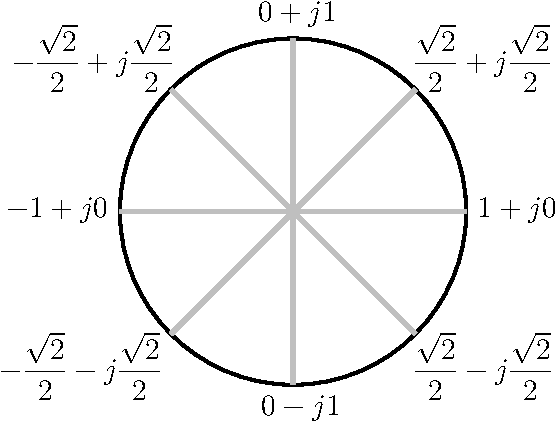
\includegraphics[width=0.3\textwidth]{img/Einheitskreis-crop.pdf}
  \caption{Einheitskreis mit relevanten Werten der 8x8-DFT}
  \label{pic:Einheitskreis_Faktoren}
\end{figure}
  
 


\begin{figure}[!ht]
 \centering
 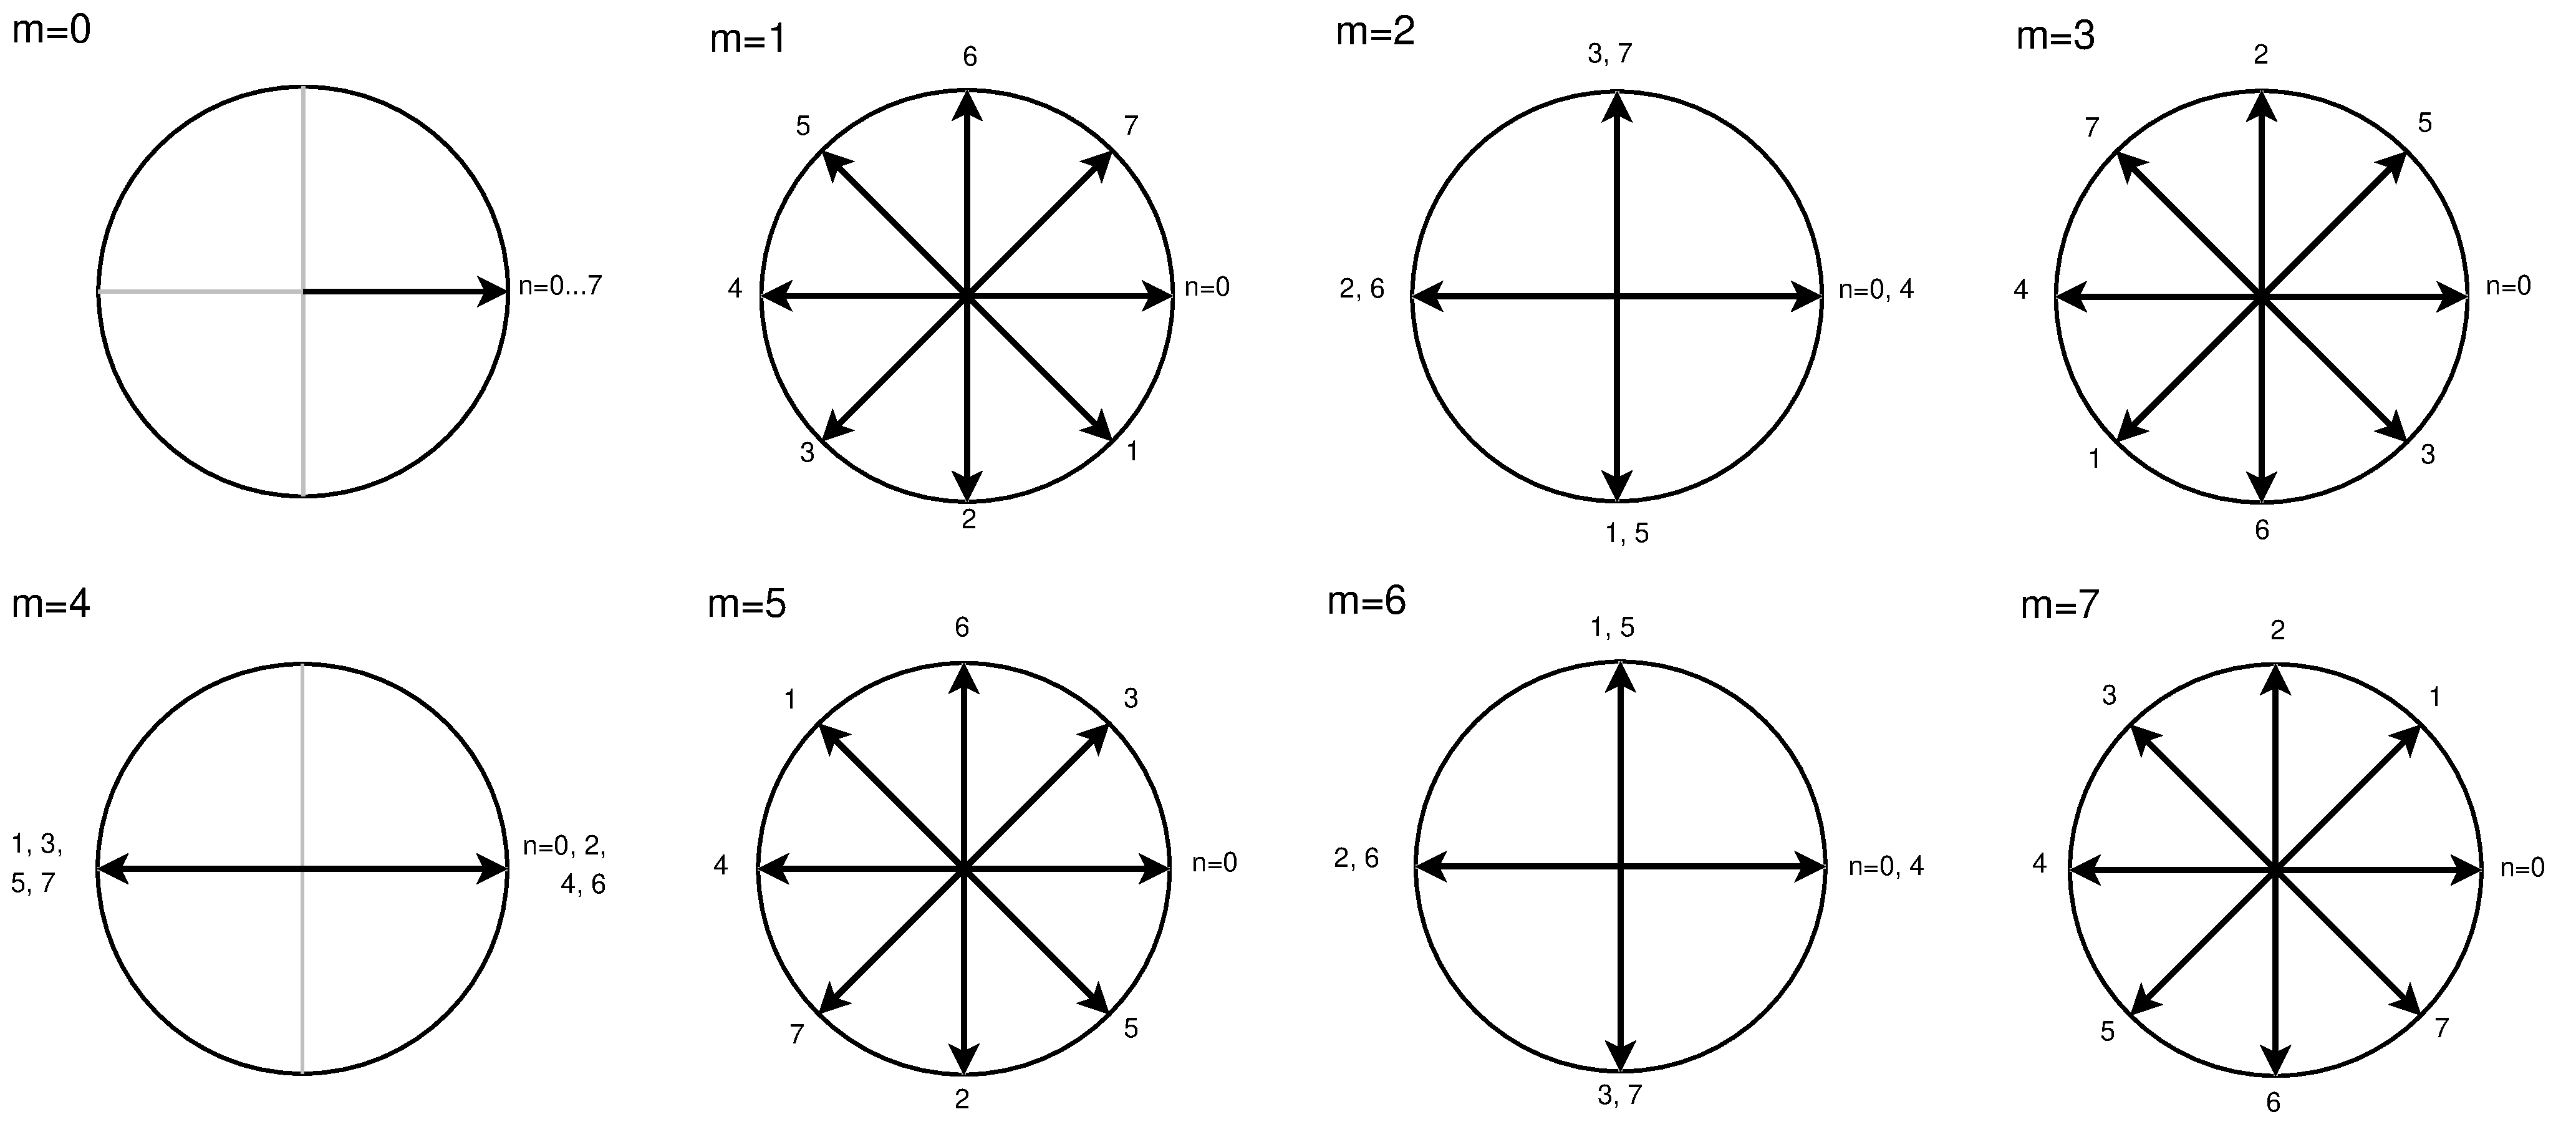
\includegraphics[width=1\textwidth]{img/Twiddlefaktoren_Einheitskreis.eps}
 \caption{Twiddlefaktoren der 8$\times$8-Matrix, aufgeteilt auf die Laufindizes $m$ und $n$. $m$ bezieht sich auf das Element im Ausgangsvektor $\vec{X}$, $n$ auf den Eingangsvektor $\vec{x}$. Siehe auch Gl. (\ref{eq:dft}).}
 \label{pic:Twiddlefaktoren_Darstellung8x8}
\end{figure}

\vspace{0.5cm}
 
 Wie anhand der Grafiken \ref{pic:Einheitskreis_Faktoren} zu sehen ist, setzen sich die Faktoren ausschließlich aus den Zahlen $\pm1$, $\pm\nicefrac{\sqrt{2}}{2}$ und $0$ 
 zusammen. Gemäß der Definition für nicht triviale Werte aus Abschnitt \ref{sec:BewertungVerschiedenerGroessen} zählt ausschließlich der letztgenannte zu diesen.
 Ebenfalls ist ersichtlich, dass der Betrag aller Zahlen immer $1$ ist.
 In Abbildung \ref{pic:MatrizenDarstellungTwiddlefaktoren} ist die Twiddlefaktormatrix auf zwei Matrizen aufgeteilt, wobei die Zahlen durch Farben repräsentiert werden.
 Die linke enthält alle realen Anteile, die rechte alle imaginären. 
 Anhand der Grafik lässt sich gut die Symmetrie erkennen, mit der die Werte auftreten. Diese Grafik soll als 
 Ausgangspunkt für die folgende Betrachtung dienen.
 Es lässt sich auch gut erkennen, das ein Kreis aus Abbildung \ref{pic:Twiddlefaktoren_Darstellung8x8} die Werte der korrespondierenden Zeilen wiederspiegelt.
 
 \begin{minipage}{0.9\textwidth}
\begingroup
 \renewcommand*{\arraystretch}{0.95} % Zeilenabstand der Tabelle

\begin{center}
  \[
   \stackrel{\mbox{$Re\{W\}$}}{
    \begin{bmatrix}
     \myboxOnePos 	& \myboxOnePos 		& \myboxOnePos 	& \myboxOnePos 		& \myboxOnePos 	& \myboxOnePos 		& \myboxOnePos 	& \myboxOnePos \\
     \myboxOnePos 	& \myboxSqrtPos 	& \myboxZero 	& \myboxSqrtNeg		& \myboxOneNeg	& \myboxSqrtNeg		& \myboxZero	& \myboxSqrtPos \\
     \myboxOnePos 	& \myboxZero 		& \myboxOneNeg 	& \myboxZero 		& \myboxOnePos 	& \myboxZero 		& \myboxOneNeg 	& \myboxZero \\
     \myboxOnePos 	& \myboxSqrtNeg 	& \myboxZero 	& \myboxSqrtPos 	& \myboxOneNeg 	& \myboxSqrtPos 	& \myboxZero 	& \myboxSqrtNeg \\
     \myboxOnePos 	& \myboxOneNeg 		& \myboxOnePos 	& \myboxOneNeg 		& \myboxOnePos 	& \myboxOneNeg 		& \myboxOnePos 	& \myboxOneNeg \\
     \myboxOnePos 	& \myboxSqrtNeg 	& \myboxZero 	& \myboxSqrtPos 	& \myboxOneNeg 	& \myboxSqrtPos 	& \myboxZero 	& \myboxSqrtNeg \\
     \myboxOnePos 	& \myboxZero 		& \myboxOneNeg 	& \myboxZero 		& \myboxOnePos 	& \myboxZero 		& \myboxOneNeg 	& \myboxZero \\
     \myboxOnePos 	& \myboxSqrtPos 	& \myboxZero 	& \myboxSqrtNeg		& \myboxOneNeg	& \myboxSqrtNeg		& \myboxZero	& \myboxSqrtPos 
    \end{bmatrix}
   }
   \hspace{1cm}
   \stackrel{\mbox{$Im\{W\}$}}{
    \begin{bmatrix}
     \myboxZero 	& \myboxZero 		& \myboxZero 	& \myboxZero 		& \myboxZero 	& \myboxZero 		& \myboxZero 	& \myboxZero \\
     \myboxZero 	& \myboxSqrtNeg 	& \myboxOneNeg 	& \myboxSqrtNeg		& \myboxZero	& \myboxSqrtPos		& \myboxOnePos	& \myboxSqrtPos \\
     \myboxZero 	& \myboxOneNeg 		& \myboxZero 	& \myboxOnePos 		& \myboxZero 	& \myboxOneNeg 		& \myboxZero 	& \myboxOnePos \\
     \myboxZero 	& \myboxSqrtNeg 	& \myboxOnePos 	& \myboxSqrtNeg 	& \myboxZero 	& \myboxSqrtPos 	& \myboxOneNeg 	& \myboxSqrtPos \\
     \myboxZero 	& \myboxZero 		& \myboxZero 	& \myboxZero 		& \myboxZero 	& \myboxZero 		& \myboxZero 	& \myboxZero \\
     \myboxZero 	& \myboxSqrtPos 	& \myboxOneNeg 	& \myboxSqrtPos		& \myboxZero 	& \myboxSqrtNeg 	& \myboxOnePos 	& \myboxSqrtNeg \\
     \myboxZero 	& \myboxOnePos 		& \myboxZero 	& \myboxOneNeg 		& \myboxZero 	& \myboxOnePos 		& \myboxZero 	& \myboxOneNeg \\
     \myboxZero 	& \myboxSqrtPos 	& \myboxOnePos 	& \myboxSqrtPos		& \myboxZero	& \myboxSqrtNeg		& \myboxOneNeg	& \myboxSqrtNeg 
    \end{bmatrix}
   }
  \]
\vspace{0.5cm}
  Legende: $\myboxOnePos$ = 1 \quad $\myboxOneNeg$ = -1 \quad $\myboxZero$ = 0 \quad $\myboxSqrtPos$ = $\nicefrac{\sqrt{2}}{2}$ \quad $\myboxSqrtNeg$ = -$\nicefrac{\sqrt{2}}{2}$
  \captionof{figure}{Matrix-Darstellung der 8x8-DFT-Twiddlefaktoren aufgeteilt nach Real- und Imaginärteil.}
  \label{pic:MatrizenDarstellungTwiddlefaktoren}
\end{center}
\endgroup
\end{minipage}


\vspace{0.5cm}
 
 Auf den ersten Blick sticht die erste Zeile hervor, da sie im Realteil nur aus positiven Einsen und im Imaginärteil nur aus Nullen besteht.
 Mit der fünften Zeile verhält es sich ähnlich. Anders ist hier, dass sich positive und negative Einsen abwechseln.
 In die gleiche Gruppe können noch die dritte und die siebte Zeile zusammengefasst werden. 
 %Beide haben gemeinsam, dass sie so wie die erste und fünfte nur Einsen und Nullen als Faktoren haben. 
 Im Unterschied zu den vorigen können hier aber auch die Imaginärteile eine positive bzw. negative Eins haben. Entsprechend ist dann der Realteil
 Null. Hier müssen zur Berechnung des Ergebnisses also auch Imaginärteile der Eingangsmatrix mit einbezogen werden.
 Für die vier bisher betrachteten Zeilen gilt, dass zur Berechnung eines Elements der Ergebnismatrix ausschließlich Additionen oder Subtraktionen erforderlich sind. 
 
 
 Alle Werte, die bis jetzt vorkamen, haben entweder nur einem Real- oder einem Imaginärteil. 
 Dies hat den Vorteil, dass weniger Berechnungen erfolgen müssen, da von einer vollständig komplexen Multiplikation nur eine Multiplikation einer komplexen Zahl mit einer
 rein reellen (bzw. imaginären) übrig bleiben. Au diese Weise reduziert sich der in Gleichungen (\ref{eq:komplexe_Multiplikation}) gezeigte Aufwand zu dem in Gleichung (\ref{eq:halb_komplexe_Multiplikation}).
 Darüber hinaus sind bei den bisherigen Zahlen keine Multiplikationen nötig, weshalb sich der Rechenaufwandt auf den Additionsteil der Gleichung beschränkt.
 
 \begin{align}\label{eq:halb_komplexe_Multiplikation}
 \begin{split}
  e + jf &= a \cdot (c + jd)\\
         &= a \cdot c + j(a \cdot d)\\
 \end{split}
 \end{align}
 
 Für die übrigen vier Zeilen gelten die bisherigen Beobachtungen nicht oder nur teilweise, weshalb sie nicht zur ersten Gruppe gezählt werden können.
 Dafür haben sie aber alle gemein, dass die Hälfte der Faktoren sowohl einen Real- als auch einen Imaginärteil besitzen, welche symmetrisch angeordnet sind.
 Für diese vier Faktoren sind deshalb jeweils die gesamten vier Multiplikationen aus Gleichung \ref{eq:komplexe_Multiplikation} nötig.

 Eine besondere Eigenschaft ist, dass der Faktor für nicht triviale Multiplikationen im Real- und Imaginärteil zumindest vom Betrag her identisch sind.
 Dies liegt daran, dass der Einheitskreis in acht Teile geteilt wird und für beispielsweise $\frac{2\cdot\pi}{8}=\frac{\pi}{4}$ der Sinus- und Kosinuswert identisch sind. 
 Hieraus resultiert, dass die Hälfte der Berechnungen der nicht trivialen Werte, die für die reelle Matrix gemacht werden müssen,
 direkt für den imaginären Anteil übernommen werden könnten. Die andere Hälfte müsste lediglich negiert werden. 
 Deshalb kann das berechnete Verhältnis von 3 in Tabelle \ref{tab:DFT-TwiddlefaktorMatrizenBewertung} als deutlich höher angenommen werden.
 


